\documentclass[11pt,a4paper]{article}

\usepackage[margin=2.6cm]{geometry}
\usepackage{amsmath}
\usepackage{amssymb}
\usepackage{graphicx}
\usepackage[hidelinks]{hyperref}

% Optional packages: the document degrades gracefully without them, so it
% compiles on a minimal TeX Live as well as on a full installation.
\IfFileExists{booktabs.sty}{\usepackage{booktabs}}{%
  \newcommand{\toprule}{\hline}
  \newcommand{\midrule}{\hline}
  \newcommand{\bottomrule}{\hline}
  \newcommand{\cmidrule}[2][]{}%
}
\IfFileExists{microtype.sty}{\usepackage{microtype}}{}

% Figure 1 is produced by make_figures.py (matplotlib) rather than TikZ, so the
% numbers in the plot come from one source and cannot drift from the text.

\newcommand{\xhat}{\hat{\mathbf{x}}}
\newcommand{\yhat}{\hat{\mathbf{y}}}
\newcommand{\zhat}{\hat{\mathbf{z}}}
\newcommand{\svec}{\mathbf{s}}
\newcommand{\gvec}{\mathbf{g}}
\newcommand{\SE}{\mathrm{SE}(3)}
\newcommand{\SO}{\mathrm{SO}}

\title{Exploiting Rigid-Body Symmetry in Flow-Matching Motion Planning:\\
       Canonicalisation Rather Than Equivariance}
\author{Andrea Sevincel}
\date{August 2026}

\begin{document}
\maketitle

\begin{abstract}
\noindent
Motion planning is equivariant under rigid transformations: translate or rotate a
planning problem and its solution transforms identically. A neural planner trained on
world coordinates does not know this and must relearn the same skill at every pose.
This report describes a method that supplies the symmetry through the \emph{problem
representation} rather than through the network architecture, and reports what it
contributes on a 3D point-mass benchmark.

The central observation is that the start and goal points themselves determine a
frame, and that this frame removes five of the six degrees of freedom of $\SE$
\emph{exactly and for free}. The sixth --- a roll about the start--goal axis --- provably
cannot be removed by any continuous rule, for two independent reasons. I therefore
handled it by symmetry: uniform roll augmentation during training and frame averaging
at inference.

On held-out environments the canonicalisation raises the collision-free rate from
$15.4\%$ to $45.6\%$, a gap of $30.2$ percentage points ($\approx 11$ standard
errors), and the advantage \emph{widens} with training data rather than shrinking.
The two mechanisms built for the sixth degree of freedom contribute nothing
measurable: $+1.2$ and $+0.2$ percentage points respectively, both inside noise.
A direct measurement explains why --- only $1.6\%$ of the learned velocity field is
non-equivariant, and that fraction \emph{decreases} as training data grows. The
practical conclusion is that the valuable operation is canonicalising the degrees of
freedom one can, and that an equivariant architecture would constrain precisely the
component that is already correct.
\end{abstract}

\section{Introduction}

A motion planning problem consists of a workspace populated with obstacles, a start
configuration $\svec$ and a goal configuration $\gvec$. Its solution is a path
$\tau$ from $\svec$ to $\gvec$ avoiding the obstacles. The problem possesses an exact
symmetry: for any rigid transformation $T \in \SE$, the solution to the transformed
problem is the transformed solution,
\begin{equation}
  \tau\bigl(T\!\cdot\!\text{obstacles},\, T\svec,\, T\gvec\bigr)
  \;=\; T \cdot \tau\bigl(\text{obstacles},\, \svec,\, \gvec\bigr).
  \label{eq:equivariance}
\end{equation}
Nothing about the physics changes when the problem is picked up and moved.

A neural planner trained on raw world coordinates has no access to
Eq.~\eqref{eq:equivariance}. As far as its weights are concerned, planning
left-to-right near the ceiling is an unrelated task from planning front-to-back near
the floor, and the same skill must be learned separately at every pose. Two remedies
exist. The first is to build the symmetry into the architecture --- constrained layers,
irreducible representations, gated nonlinearities --- which is expensive to implement,
introduces a class of bugs that fail silently, and costs expressiveness. The second
is to build it into the \emph{representation of the problem}, so that the network is
never shown the pose at all and therefore cannot be sensitive to it. This report
pursues the second.

The contribution is threefold. First, a decomposition of $\SE$ for this problem class
that separates the five degrees of freedom removable by canonicalisation from the one
that is not, with a proof that the remaining one is not removable by \emph{any}
continuous rule. Second, a measurement of what each mechanism contributes, rather
than a demonstration that the combination works. Third, a negative result reported
quantitatively: the symmetry machinery for the sixth degree of freedom is inert on
this problem, and I measured \emph{how much} non-equivariance existed in order to say
so with confidence rather than by observing flat quality curves.

\section{Background}

\subsection{The benchmark}

Experiments use PointMass3D, a benchmark I built in the earlier stage of this
internship. A spherical robot of radius $0.03$ moves in the workspace $[-1,1]^3$
populated with $20$ spheres and $20$ axis-aligned boxes per environment, with obstacle
centres drawn uniformly in $[-0.75, 0.75]^3$. Collision checking uses an analytic
signed distance field: the environment SDF is the minimum over all obstacle SDFs and
the workspace walls, and clearance subtracts the robot radius. Start and goal are
drawn uniformly in the workspace subject to a collision margin and a minimum
separation $\|\gvec - \svec\| \ge 1.5$.

Expert demonstrations come from a pipeline of RRT-Connect for an initial feasible
path, random shortcutting, uniform resampling to $64$ waypoints, and CHOMP refinement.
The dataset used here contains $300$ environments $\times$ $600$ start--goal pairs
$\times$ $30$ trajectories, doubled by time-reversal, for $10.8$M paths.

\subsection{The flow-matching planner}

The learned planner is a conditional flow-matching model over whole trajectories,
following the rectified-flow / conditional-OT formulation. A trajectory is represented
as $N=64$ waypoints in $\mathbb{R}^3$. Training draws $\mathbf{x}_0 \sim
\mathcal{N}(0, I)$, $t \sim \mathcal{U}[0,1]$, forms the interpolant
$\mathbf{x}_t = (1-t)\mathbf{x}_0 + t\,\mathbf{x}_1$ with $\mathbf{x}_1$ an expert
trajectory, and regresses the velocity target $\mathbf{x}_1 - \mathbf{x}_0$:
\begin{equation}
  \mathcal{L} = \mathbb{E}_{\mathbf{x}_0, \mathbf{x}_1, t}
  \bigl\| v_\theta(\mathbf{x}_t, t, c) - (\mathbf{x}_1 - \mathbf{x}_0) \bigr\|^2 ,
\end{equation}
where $c$ encodes the obstacles and the query. Sampling integrates
$\dot{\mathbf{x}} = v_\theta(\mathbf{x}, t, c)$ from $t=0$ to $t=1$ with explicit
Euler steps. The network is a dilated temporal convolutional trunk with FiLM
conditioning, fed by a PointNet-style permutation-invariant obstacle encoder;
$2.16$M parameters in the configuration used throughout.

\section{Method}

\subsection{Decomposing the symmetry group}

$\SE$ has six degrees of freedom: three translations and three rotations. The key
observation is that the query itself supplies a frame, and that this frame consumes
five of them.

\begin{itemize}
  \item \textbf{Three translations} are removed by placing the origin at the midpoint
  $\tfrac{1}{2}(\svec + \gvec)$.
  \item \textbf{Two of the three rotations} are removed by aligning the first axis
  with the start--goal direction $\xhat = (\gvec - \svec)/\|\gvec - \svec\|$.
  Specifying a direction on the sphere $S^2$ costs exactly two degrees of freedom, so
  fixing one axis to it spends two.
  \item \textbf{One rotation remains}: the roll about $\xhat$. Having fixed which way
  the path runs, nothing in the problem specifies which way is ``up'' around that axis.
\end{itemize}

The five removable degrees of freedom yield \emph{exact} equivariance, not an
approximation, and this deserves emphasis. The frame is computed from the query. Under
a rigid transformation $T$, the points $\svec$ and $\gvec$ transform with the problem,
so the frame transforms with them and the reduced-frame representation is
\emph{bit-identical}. The network never observes the pose; it cannot be sensitive to
something it is not shown. This is a stronger guarantee than any trained architecture
provides, and it holds to floating-point precision.

\subsection{Why the sixth degree of freedom is not removable}

One might hope to fix the roll by some rule. It cannot be done, and the obstruction is
structural rather than a deficiency of any particular construction.

\paragraph{Obstruction from geometry.} A rule assigning a ``up'' direction
$\yhat(\xhat)$ perpendicular to each axis direction is precisely a continuous,
nowhere-vanishing unit tangent vector field on $S^2$. The hairy ball theorem forbids
the existence of such a field. Every deterministic gauge therefore has a
discontinuity; one may relocate it but never eliminate it. The domain here is the
whole sphere --- axis-aligned start--goal directions require a displacement of at
least $1.5$ along one axis out of the $2.0$ available, so no direction is excluded ---
and hence there is no escape via a contractible subdomain.

\paragraph{Obstruction from the scene.} One might instead derive the roll from the
obstacle field, for instance from the angular first moment
$c_1 = \sum_j w_j e^{i\varphi_j}$ of the obstacle centres projected into the plane
normal to $\xhat$. This also fails. Obstacle centres are drawn uniformly in a cube,
which is $4$-fold symmetric in any coordinate plane; a $C_4$-invariant distribution has
vanishing Fourier coefficients at every order $m \not\equiv 0 \pmod 4$. Hence
$\mathbb{E}[c_1] = 0$ \emph{and} $\mathbb{E}[c_2] = 0$ identically. Under this null,
$|c_1|^2/\sum_j w_j^2$ is $\mathrm{Exp}(1)$-distributed with median $\approx 0.69$, so
near-degenerate configurations are not a rare tail but the typical case. The first
surviving moment, $m=4$, is an artefact of cube sampling, is fourfold ambiguous by
construction, and would not transfer to a realistic scene distribution.

Both routes are closed, for unrelated reasons. The sixth degree of freedom must
therefore be handled by symmetry rather than canonicalisation.

\subsection{The $(\svec,\gvec)$ reduction}

The reduction maps world coordinates to a canonical frame. Given a query, let
\begin{align}
  \mathbf{o} &= \tfrac{1}{2}(\svec + \gvec), &
  \xhat &= \frac{\gvec - \svec}{\|\gvec - \svec\|}, &
  d &= \|\gvec - \svec\| .
\end{align}
The remaining two axes come from crossing $\xhat$ with whichever coordinate axis it is
least aligned with, $\yhat \propto \xhat \times \mathbf{e}_{i^\ast}$ where
$i^\ast = \arg\min_i |\xhat_i|$, and $\zhat = \xhat \times \yhat$. Because the
smallest component of a unit vector satisfies $|\xhat_{i^\ast}| \le 1/\sqrt{3}$, this
cross product has norm $\ge \sqrt{2/3} \approx 0.816$ everywhere, so the construction
is well-conditioned over the entire domain with no threshold or fallback case. The
rotation $R$ has these three vectors as rows, so reduced coordinates are
$R(\mathbf{p} - \mathbf{o})$, and $\det R = +1$ by construction.

Two consequences follow immediately. Start and goal always map to
$(\mp d/2, 0, 0)$, so the six numbers previously used to condition the network collapse
to the single invariant scalar $d$. And every pair of training examples that were ``the
same problem in a different pose'' now coincide, which increases the effective density
of the training set without generating anything.

\subsection{Roll augmentation and frame averaging}

For the residual roll I implemented two standard mechanisms.

\textbf{Roll augmentation.} During training a uniform angle $\theta \sim
\mathcal{U}[0, 2\pi)$ is composed into the same rotation matrix, so the reduction and
the roll are applied as a single transformation rather than two. The Gaussian prior
$\mathbf{x}_0$ is drawn \emph{after} this rotation and is never rotated: an isotropic
Gaussian is already rotation-invariant, so rotating it would be a redundant step
capable only of introducing error.

\textbf{Frame averaging.} At inference the velocity field is evaluated at $K$ rolled
copies of the state, each result rotated back, and the results averaged:
\begin{equation}
  \bar{v}(\mathbf{x}) = \frac{1}{K} \sum_{k=0}^{K-1}
  \rho(\theta_k)^{-1} f\bigl(\rho(\theta_k)\,\mathbf{x}\bigr),
  \qquad \theta_k = \frac{2\pi k}{K} .
  \label{eq:fa}
\end{equation}
For $\alpha = 2\pi j / K$ this operator is \emph{exactly} $C_K$-equivariant regardless
of $f$: rolling the input by $\alpha$ permutes the quadrature points, and reindexing a
finite sum is a bijection on them. No architectural constraint or training assumption
is required; the guarantee is a property of the operator. Because the obstacle encoding
is time-independent, the $K$ rolled scene encodings are computed once outside the ODE
loop and reused at every integration step.

\subsection{Implementation}

Three changes were required to make the reduction representable, and one class of
error had to be designed out.

\paragraph{Oriented boxes.} The reduction is a general $\SO(3)$ rotation, under which
an axis-aligned box becomes an oriented box. The original six-number representation
(centre and half-extents) cannot express this. I replaced it with a twelve-dimensional
representation: a centre and three half-edge \emph{vectors}. In the world frame these
are $(h_x,0,0)$, $(0,h_y,0)$, $(0,0,h_z)$, so the re-encoding is lossless. Note that
the environment SDF is unchanged: collision checking occurs in the world frame after
the inverse transform, so no oriented-box distance function is needed.

\paragraph{Points and free vectors transform differently.} This is the error the
implementation is principally designed to prevent, because it fails silently.
Waypoints, endpoints, and obstacle centres are \emph{points} and take the full affine
map $R(\mathbf{p} - \mathbf{o})$. The three box half-edges are \emph{free vectors} and
take the rotation only, $R\mathbf{v}$. Applying the affine map to a half-edge
introduces the error $-R\mathbf{o}$ on every edge --- identically, as one can verify
--- so box \emph{position} survives while box \emph{extent} is swamped by a common
offset. The model becomes blind to obstacle size while the loss curve remains
healthy. The severity scales with $\|\tfrac{1}{2}(\svec+\gvec)\|$, so the defect is
invisible on problems whose endpoints straddle the origin, which makes it harder still
to detect empirically.

\paragraph{Verification.} I wrote eighteen tests covering deliberately disjoint failure
classes. Asserting that $\svec, \gvec$ land on $(\mp d/2, 0, 0)$ catches translation
errors, axis ordering, and $R$ versus $R^\top$, but is blind to handedness, because a
reflection in the $y$--$z$ plane fixes the $x$-axis pointwise; $\det R > 0$ covers
that. Neither detects the point/vector confusion, so a third test asserts
$\mathrm{featurise}(\rho \cdot S) = \mathrm{typed\_rotate}(\mathrm{featurise}(S), \rho)$
with the reference side written as explicit loops rather than the batched operations
under test, so that it catches indexing and reshaping errors instead of agreeing with
them. A separate suite verifies that Eq.~\eqref{eq:fa} is exactly $C_K$-equivariant
against a deliberately \emph{untrained} network --- the hard case, since the guarantee
should not depend on $f$.

One subtlety is worth recording. The group acts on the whole input, scene and state
together. An early version of the equivariance test rolled only the state while
leaving the conditioning attached to its original frame, which produced a large
apparent violation from a correct implementation. A diagnostic written that way would
report non-equivariance that is not present.

\section{Experiments}

\subsection{Protocol}

All figures use environments $250$--$299$ of the $300$-environment dataset, which no
model was trained on, evaluated as $50$ environments $\times$ $10$ start--goal pairs
$\times$ $20$ samples with $8$ Euler steps. The two arms are:

\begin{description}
  \item[Control] world frame, conditioned on the raw pair $(\svec, \gvec)$.
  \item[Treatment] the $(\svec,\gvec)$ reduction with uniform roll augmentation,
  conditioned on the invariant scalar $d$.
\end{description}

Both arms use the twelve-dimensional oriented-box representation so that it is not a
confound. Within the training environments, validation holds out whole start--goal
pairs; a per-trajectory split leaks badly on this dataset, because the $30$
trajectories per pair are near-duplicates (within-pair standard deviation $0.054$
against an overall $0.426$, since CHOMP is a local optimiser and converges to the same
route from similar initialisations). Under a per-trajectory split a held-out
trajectory has a training neighbour at RMS distance $0.030$; under the pair split this
rises to $0.162$.

Statistical statements treat the number of \emph{distinct problems} ($500$) as the
sample size rather than the number of trajectories ($10{,}000$), since samples within
a problem and problems within an environment are correlated. This gives a standard
error of roughly $2$ percentage points.

Validation loss is \emph{not} comparable across arms: the treatment regresses targets
in the reduced frame, where trajectories are canonicalised along $+\xhat$, so its
target variance and hence its mean squared error are mechanically smaller. All
reported quantities are therefore world-frame.

\subsection{Main result: the reduction scales, the baseline does not}

\begin{table}[t]
\centering
\begin{tabular}{lrrrr}
\toprule
& \multicolumn{2}{c}{Collision-free (\%)} & \multicolumn{2}{c}{Min.\ clearance} \\
\cmidrule(lr){2-3}\cmidrule(lr){4-5}
Training environments & Control & Treatment & Control & Treatment \\
\midrule
20  & 12.8 & 19.0 & $-0.0776$ & $-0.0583$ \\
60  & 13.5 & 31.3 & $-0.0746$ & $-0.0312$ \\
150 & 14.6 & 41.0 & $-0.0726$ & $-0.0163$ \\
250 & 15.4 & \textbf{45.6} & $-0.0697$ & $\mathbf{-0.0095}$ \\
\bottomrule
\end{tabular}
\caption{Held-out performance against training-set size. The control gains $2.6$
percentage points across a $12.5\times$ increase in environments; the treatment gains
$26.6$ and has not plateaued.}
\label{tab:main}
\end{table}

\begin{figure}[t]
\centering
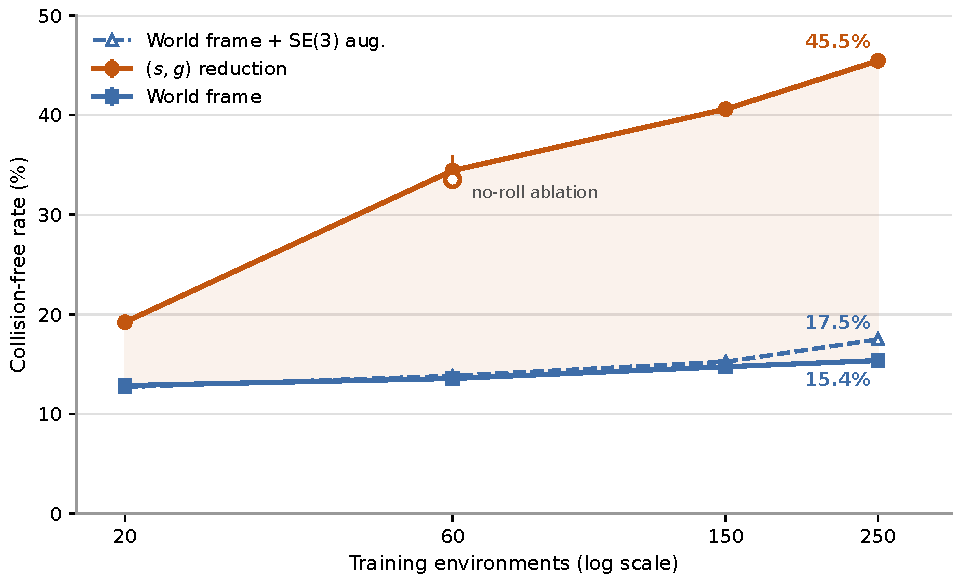
\includegraphics[width=0.82\textwidth]{fig_scaling.pdf}
\caption{The gap widens with data. If the reduction were compensating for a shortage
of training data one would expect it to close; instead the world-frame baseline is
nearly flat while the reduced model continues to improve. The hollow marker is the
no-roll ablation, drawn on the treatment line because it is the same arm with one
component removed. Shaded region marks the gap between the arms.}
\label{fig:scaling}
\end{figure}

Table~\ref{tab:main} and Figure~\ref{fig:scaling} give the principal result. At $250$
environments the reduction reaches $45.6\%$ against the baseline's $15.4\%$, a gap of
$30.2$ percentage points. Taking the standard error of the difference as
$\approx 2.7$ points, this is roughly $11$ standard errors.

The more informative feature is the \emph{trend}. The baseline improves by only $2.6$
points across a $12.5\times$ increase in the number of training environments; it is
close to unable to exploit additional layouts. The treatment improves by $26.6$ points
over the same range and has not levelled off. This is the opposite of what one would
observe if canonicalisation were a small-data expedient, in which case the advantage
should shrink as data accumulates. Minimum clearance corroborates the conclusion
through an independent, continuous measure: the treatment moves from $-0.058$ toward
$-0.0095$, approaching feasibility, while the baseline is essentially static.

Endpoint error falls by a factor of three to five under the reduction ($0.0101 \to
0.0041$ at $20$ environments, $0.0059 \to 0.0020$ at $250$). This is a direct
consequence of canonicalisation: with endpoints always at $(\mp d/2, 0, 0)$ the model
no longer expends capacity on \emph{where} they are.

\subsection{The mechanisms for the sixth degree of freedom are inert}

\begin{table}[t]
\centering
\begin{tabular}{lrl}
\toprule
Mechanism & Contribution & Assessment \\
\midrule
$(\svec,\gvec)$ reduction (5 DOF) & $+30.2$ pp & $\approx 11$ SE; grows with data \\
Roll augmentation                 & $+1.2$ pp  & inside noise \\
Frame averaging ($K{=}1 \to 9$)   & $+0.2$ pp  & $0.09$ SE; indistinguishable from zero \\
\bottomrule
\end{tabular}
\caption{Decomposition of the benefit by mechanism, all measured on the same held-out
set. The entire effect is attributable to canonicalisation.}
\label{tab:ablation}
\end{table}

Table~\ref{tab:ablation} decomposes the result. Removing roll augmentation
(training with the reduction but a fixed gauge) costs $31.3\% \to 30.1\%$ at $60$
environments, inside noise. Frame averaging on the best model gives
$45.6 / 45.7 / 45.8\%$ for $K = 1, 3, 9$: a change of $0.2$ points, or $0.09$ standard
errors.

Rather than infer inertness from flat quality curves, I measured the quantity frame
averaging is designed to remove. The non-equivariance residual
\begin{equation}
  r = \frac{\mathbb{E}\bigl\|v_k - \bar{v}\bigr\|}{\|\bar{v}\|}
\end{equation}
is the disagreement among the $K$ rotated estimates. On the best model $r = 0.0157$ at
$K=3$ and $0.0174$ at $K=9$: under $2\%$ of the velocity field is non-equivariant.
Since Eq.~\eqref{eq:fa} is the orthogonal projection onto the equivariant subspace, it
can remove \emph{only} that $2\%$. The remaining error --- and with the model at
$45.6\%$ collision-free there is a great deal of it --- respects the symmetry and is
untouchable by symmetrisation.

Two further observations sharpen this. First, the residual barely moves when roll
augmentation is removed, so augmentation was not the cause of the near-equivariance.
The explanation is that the gauge is a deterministic function of $\xhat$, and $600$
start--goal pairs per environment supply $600$ distinct directions; the reduced-frame
training data already spans a wide spread of rolls, and explicit augmentation was
addressing a problem the data had already solved. Second, the residual \emph{decreases}
with scale, from $0.0186$ at $60$ training environments to $0.0157$ at $250$. The model
becomes more equivariant as it observes more layouts.

The second observation is the strongest available argument against an equivariant
architecture. The property such an architecture would enforce by construction is
emerging on its own and strengthening with data, so imposing it would trade
expressiveness for something obtained free of charge.

\subsection{Cost}

Frame averaging at $K=9$ costs $1.05\times$ the wall-clock time of $K=1$
($0.070$ vs $0.067$ s per query). At $64$ waypoints and batch size $1$ the sampler is
bound by kernel launch overhead rather than arithmetic, so the ninefold increase in
width is nearly free. This matters for the interpretation: the finding that frame
averaging does not help is not a budget trade-off, since it was affordable and was
adopted anyway for the measurement.

Separately, reducing the integrator from $20$ to $8$ Euler steps costs $0.4$--$0.8$
percentage points and runs $1.4\times$ faster, so $8$ steps is used throughout.

\section{Discussion}

\subsection{What the technique contributes}

The contribution is best stated as a decomposition rather than a single number. Of the
six degrees of freedom of $\SE$, five can be removed exactly by a frame constructed
from the query, at no computational cost and with no architectural constraint. Doing so
roughly triples the collision-free rate on this benchmark and, more importantly,
converts a model that cannot use additional training environments into one that can.

The sixth degree of freedom cannot be removed, and --- on this problem --- does not need
to be. That is a contingent empirical fact rather than a theorem, but it is supported
by three independent measurements: the ablation, the $K$ sweep, and the direct residual.

The methodological point I would emphasise is the value of measuring the residual. Had
I only observed that frame averaging left quality unchanged, the honest conclusion
would have been ``it did not help here'', which is weak. Measuring that only $1.6\%$ of
the field is non-equivariant converts this into a statement about \emph{why}, and
supports the stronger claim that no symmetrisation method --- including an equivariant
architecture --- can recover more than that.

\subsection{What the results do not say}

The absolute performance is poor. A workspace containing forty obstacles is dense, and
the model is small ($2.16$M parameters) and briefly trained ($20$ epochs). No
train--validation gap appeared in any run, indicating the models are underfitting; the
comparison between arms is sound, but the level indicates substantial headroom in
capacity and training budget.

The claim that the sixth degree of freedom needs no treatment is specific to this
setting. It relies on the training distribution supplying implicit roll diversity via
many start--goal directions. A dataset with few directions per environment, or a task
whose angular structure is genuinely richer, could plausibly reverse it. The
mechanisms remain implemented and are enabled by a flag.

Frame averaging does consistently improve endpoint error, by roughly $35\%$
($0.0020 \to 0.0013$), on every checkpoint tested. This is a real effect; it simply
does not propagate to the collision-free rate, because endpoint precision was not the
failure mode.

Finally, the dataset is markedly less diverse than its nominal size suggests. The $30$
trajectories per start--goal pair are near-duplicates, so $10.8$M paths carry on the
order of $360$k distinct queries. This does not affect the comparison, since both arms
train on identical data, but it bears on how additional data should be generated.

\subsection{Future work}

The scaling curve has not plateaued at $250$ environments, which is the maximum
available with $50$ held out. The duplication finding indicates how to afford more:
reducing the number of trajectories per pair from $30$ to $5$ would buy roughly six
times the environments for the same generation time, and environments are the binding
constraint according to Figure~\ref{fig:scaling}.

Two other directions follow from the absence of a train--validation gap. Capacity and
training length are untested levers and can be evaluated cheaply at $60$ environments.
More substantially, the flow currently begins from an isotropic Gaussian that knows
nothing of the query, so it must learn both to produce a path and to place its
endpoints. A Brownian-bridge prior pinned at start and goal would leave only the
obstacle-avoidance detour to be learned. This was previously excluded because such a
prior is not isotropic in the plane normal to $\xhat$ and would break the
distributional equivariance guarantee at $t=0$; since that guarantee has been measured
to be worth nothing here, the option is now available.

\section{Conclusion}

The model is exactly $\SE$-equivariant by construction for five of the six degrees of
freedom, and measured to be approximately $98\%$ equivariant for the sixth without any
mechanism enforcing it. All of the measured benefit lies in the five.

The practical recommendation is correspondingly simple: canonicalise the degrees of
freedom that admit a continuous canonical form, and verify by direct measurement
whether the remainder requires treatment before building machinery for it. On this
problem it did not. The result is a canonicalisation result rather than an equivariance
one, and it is more useful for being less elaborate --- the requirement is not a
specialised architecture but a discipline of not showing the network information it
should not have.

\end{document}
